\subsection{Гранаты и взрывы}
\paragraph{}
В историях всегда найдется место бутылкам с горючей смесью, емкостями с едкими летучими веществами и старым добрым гранатам. И это, и многое другое можно метнуть во врага. А потом наблюдать с безопасного расстояния, как он мечется в бессильных попытках погасить пламя, истекает кровью, изрешеченный осколками… или как бутыль предательски падает в траву, а отсыревший запал гаснет.
\paragraph{}
Гранаты — Метательное оружие с БПв = \textbf{|МСл — 2|} на Ближней и \textbf{|МСл — 4|} на Дальней дистанции. Непосредственно удар гранаты имеет Дробящие Пв и наносит КУ при выпадении 20. Используйте Мт, чтобы определить, поразил ли герой цель. Не забывайте, что гранаты можно метать в землю, поражая Зщ 10, если только герой не собирается нанести Повреждения самим броском!
\newline
Все бомбы и гранаты считаются одним видом оружия.
\paragraph{}
В случае промаха граната все равно взорвется (если только не выпала Осечка). Граната отклоняется на Х метров, где Х равен промаху героя по Зщ цели — ловкий противник может успеть отбросить гранату, а бронированный — отбить щитом или латным рукавом! Определите направление, в котором отклонилась граната, при помощи броска К20. В этом случае граната может пролететь большее расстояние, чем максимальная дистанция броска!
\begin{center}
\begin{tabular}{ |p{2.7cm}|p{12cm}| }
\hline
\textbf{К20} & \textbf{Направление}
\\ \hline
1-5 & Граната перелетела за цель
\\ \hline
6-10 & Граната отклонилась вправо от цели
\\ \hline
11-15 & Граната недолетела до цели
\\ \hline
16-20 & Граната отклонилась влево от цели
\\ \hline
\end{tabular}
\end{center}
\begin{tcolorbox}
Если нужно больше детализации по направлению, можно использовать принцип дартс: область вокруг цели делится на 20 равных секторов и каждому из них сопоставляется число, которое определяет направление отклонения.
\newline
\begin{center}
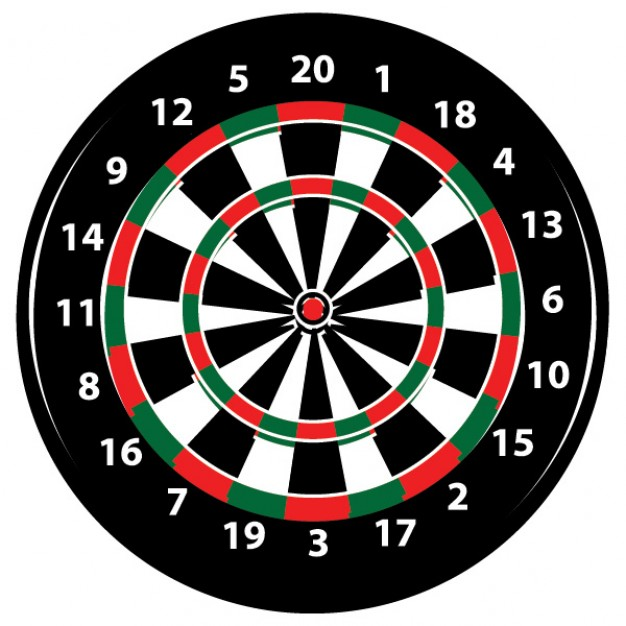
\includegraphics[width=0.5\textwidth]{darts}
\end{center}
\end{tcolorbox}
\paragraph{Вес} представленных гранат равен 0.5.
\paragraph{Дистанция} у гранат обычно Ближняя 5, Дальняя 20.
\paragraph{Центр Взрыва:} точка, из которой распространяется Взрыв.
\paragraph{Радиус Взрыва(РВ):} число метров, на которое распространяется Взрыв из центра Взрыва во все стороны. Если атака обладает свойством «Взрыв», то цель, против которой совершается проверка Доблести или Меткости, также считается находящейся в области Взрыва и получает Повреждения и прочие эффекты и от него тоже!
\paragraph{Сила Взрыва(СВ):} все существа, попавшие в радиус Взрыва, получают Пв, равные \textbf{|Сила Взрыва — БАЗщ — БДЗщ|}.
\paragraph{Газ:} газ распространяется в радиусе Взрыва и остается там какое-то время. Для определения длительности действия газа совершите проверку Неприятностей. Существа, вдохнувшие газ, страдают от эффектов яда, громко кашляют и чихают, если они еще в состоянии кашлять и чихать. Существа, имеющие Иммунитет к Ядовитым Пв, не подпадают под действие газа. В помещении увеличьте временные промежутки вдвое.
\trouble
{Штиль}%no sweat name
{Газ рассеивается чере 10 минут}%no sweat description
{Бриз}%tough day name
{Газ рассеивается через 5 минут}%tough day description
{Порыв ветра}%we have trouble name
{Газ рассеивается через 1 минуту}%we have trouble description
{Шторм}%fiasco name
{Газ рассеивается по истечении полного Круга}%fiasco description

\paragraph{Другие опасности Взрывов:} Взрывы опасны не только Повреждениями. Попавшие во Взрыв доспехи, щиты и прочие предметы, закрепленные на теле попавшего во Взрыв, получают \textbf{|Пв = Сила Взрыва — Прч|} и могут быть уничтожены. Если Взрыв достаточно силен, попавшие в него существа с воплями разлетаются в разные стороны! Если существо получает Повреждения от взрыва, его отбрасывает от центра Взрыва на \textbf{|Сила Взрыва — МСл отброшенного — МЛв отброшенного|} метров. Отброшенный получает столько Пв, сколько метров пролетел. Когда отброшенный сталкивается с другим существом, оно падает, если \textbf{|Сл отброшенного + БДЗщ отброшенного + БЩЗщ отброшенного $\pm$ БШР отброшенного| $\geq$ |Зщ существа + МСл существа $\pm$ Прч существа $\pm$ БШР существа|}. Существо получает 1 Пв за каждую единицу разницы не в свою пользу. В противном случае Пв получает отброшенный. Существо не может быть отброшено на большее число метров, чем получило Пв от Взрыва. Увеличьте расстояние броска в 2 раза за каждую категорию размера меньше Среднего и уменьшите в 2 раза за каждую категорию больше Среднего. Падения и столкновения наносят Дробящие Пв.
\newline
Если при подсчете дистанции отбрасывания получилось 0 или меньше, существо остается на месте.
